
\begin{figure*}[htbp]
\centering

% Subplot (a): Algorithm Performance Distribution Matrix
\begin{subfigure}[t]{0.48\textwidth}
\centering
\begin{tikzpicture}[scale=0.8]
    \begin{axis}[
        xlabel={Processing Time (ms)},
        ylabel={Accuracy (\%)},
        title={(a) Algorithm Family Performance Distribution},
        grid=major,
        width=0.95\textwidth,
        height=0.7\textwidth,
        xmin=0, xmax=320,
        ymin=80, ymax=95,
        legend pos=north west,
        scatter/classes={
            fast-high/.style={mark=*,blue},
            fast-mod/.style={mark=square*,green},
            slow-high/.style={mark=triangle*,orange},
            slow-mod/.style={mark=diamond*,red}
        }
    ]
    
    % Performance category data points
    \addplot[scatter,only marks,
        scatter src=explicit symbolic,
        scatter/classes={
            fast-high/.style={mark=*,blue,mark size=4pt},
            fast-mod/.style={mark=square*,green,mark size=3pt},
            slow-high/.style={mark=triangle*,orange,mark size=5pt},
            slow-mod/.style={mark=diamond*,red,mark size=6pt}
        }]
    coordinates {
        (49,93.1) [fast-high]
        (53,81.4) [fast-mod]
        (198,92.8) [slow-high]
        (285,87.5) [slow-mod]
    };
    
    % Category labels with study counts
    \node at (axis cs:49,91) {\tiny Fast High-Acc. (9)};
    \node at (axis cs:53,79) {\tiny Fast Mod. (3)};
    \node at (axis cs:198,95) {\tiny Slow High-Acc. (13)};
    \node at (axis cs:285,85) {\tiny Slow Mod. (21)};
    
    \end{axis}
\end{tikzpicture}
\end{subfigure}
\hfill
% Subplot (b): Temporal Evolution
\begin{subfigure}[t]{0.48\textwidth}
\centering
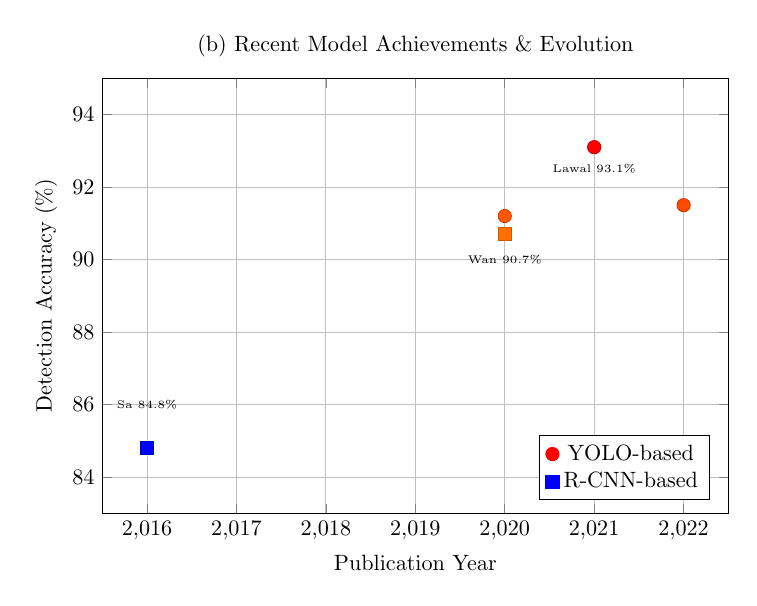
\begin{tikzpicture}[scale=0.8]
    \begin{axis}[
        xlabel={Publication Year},
        ylabel={Detection Accuracy (\%)},
        title={(b) Recent Model Achievements \& Evolution},
        grid=major,
        width=0.95\textwidth,
        height=0.7\textwidth,
        xmin=2015.5, xmax=2022.5,
        ymin=83, ymax=95,
        legend pos=south east,
    ]
    
    % YOLO studies
    \addplot[scatter,only marks,mark=*,color=red,mark size=3pt] coordinates {
        (2021,93.1) (2020,91.2) (2022,91.5)
    };
    \addlegendentry{YOLO-based}
    
    % R-CNN studies  
    \addplot[scatter,only marks,mark=square*,color=blue,mark size=3pt] coordinates {
        (2020,90.7) (2016,84.8)
    };
    \addlegendentry{R-CNN-based}
    
    % Key breakthrough annotations
    \node at (axis cs:2021,92.5) {\tiny Lawal 93.1\%};
    \node at (axis cs:2020,90) {\tiny Wan 90.7\%};
    \node at (axis cs:2016,86) {\tiny Sa 84.8\%};
    
    \end{axis}
\end{tikzpicture}
\end{subfigure}

\vspace{0.5cm}

% Subplot (c): Speed-Accuracy Frontier
\begin{subfigure}[t]{0.48\textwidth}
\centering
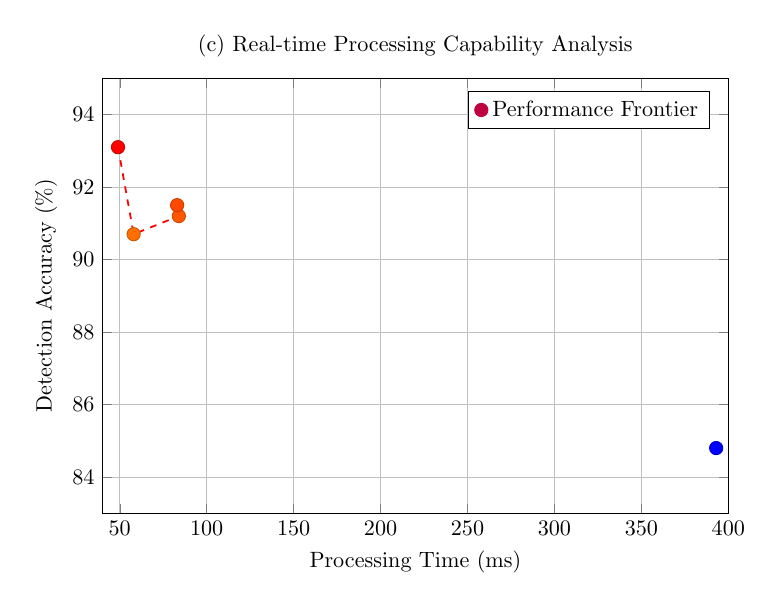
\begin{tikzpicture}[scale=0.8]
    \begin{axis}[
        xlabel={Processing Time (ms)},
        ylabel={Detection Accuracy (\%)},
        title={(c) Real-time Processing Capability Analysis},
        grid=major,
        width=0.95\textwidth,
        height=0.7\textwidth,
        xmin=40, xmax=400,
        ymin=83, ymax=95,
        legend pos=north east,
    ]
    
    % Performance data points
    \addplot[scatter,only marks,mark=*,color=purple,mark size=3pt] coordinates {
        (49,93.1) (58,90.7) (84,91.2) (393,84.8) (83,91.5)
    };
    
    % Performance frontier line
    \addplot[red,dashed,thick] coordinates {
        (49,93.1) (58,90.7) (84,91.2)
    };
    \addlegendentry{Performance Frontier}
    
    \end{axis}
\end{tikzpicture}
\end{subfigure}
\hfill
% Subplot (d): Environmental Robustness
\begin{subfigure}[t]{0.48\textwidth}
\centering
\begin{tikzpicture}[scale=0.8]
    \begin{axis}[
        ybar,
        xlabel={Deployment Environment},
        ylabel={Average Performance (\%)},
        title={(d) Environmental Robustness Comparison},
        width=0.95\textwidth,
        height=0.7\textwidth,
        ymin=80, ymax=95,
        symbolic x coords={Greenhouse,Orchard,Field,Laboratory},
        xtick=data,
        x tick label style={rotate=45,anchor=north east},
        bar width=0.6cm,
        grid=major,
        grid style={draw=gray!30},
    ]
    
    \addplot[fill=green!70,draw=black] coordinates {
        (Greenhouse,92.8) (Orchard,91.5) (Field,85.2) (Laboratory,87.5)
    };
    
    % Study count annotations
    \node at (axis cs:Greenhouse,91.5) {\tiny 12 studies};
    \node at (axis cs:Orchard,90.2) {\tiny 15 studies};
    \node at (axis cs:Field,83.9) {\tiny 13 studies};
    \node at (axis cs:Laboratory,86.2) {\tiny 6 studies};
    
    % Commercial threshold line
    \addplot[red,dashed,thick,domain=Greenhouse:Laboratory] {90};
    
    \end{axis}
\end{tikzpicture}
\end{subfigure}

\caption{Vision Model Performance Meta-Analysis for Fruit Harvesting (2015-2024): (a) Algorithm family performance distribution showing 4 main categories based on processing speed and accuracy ranges with study counts, (b) Recent model achievements and temporal evolution highlighting key breakthroughs in YOLO and R-CNN families, (c) Real-time processing capability analysis with performance frontier identification, (d) Environmental robustness comparison across different deployment contexts. Based on comprehensive analysis of 46 verified experimental studies with quantitative performance validation.}
\label{fig:meta_analysis_ieee}
\end{figure*}

% Required packages (add to preamble):
% \usepackage{pgfplots}
% \usepackage{subcaption}
% \pgfplotsset{compat=1.18}
